\section{El proceso de reciclaje y reutilización}

El proceso de reciclaje y reutilización de la e-basura no es sencillo. Es una combinación de procesos manuales y automáticos y resulta complicado organizar un proceso industrializado eficiente para la realización del proceso completo. A continuación puede verse un diagrama de flujo con las diferentes etapas del proceso:

\begin{figure}[H]
\begin{center}
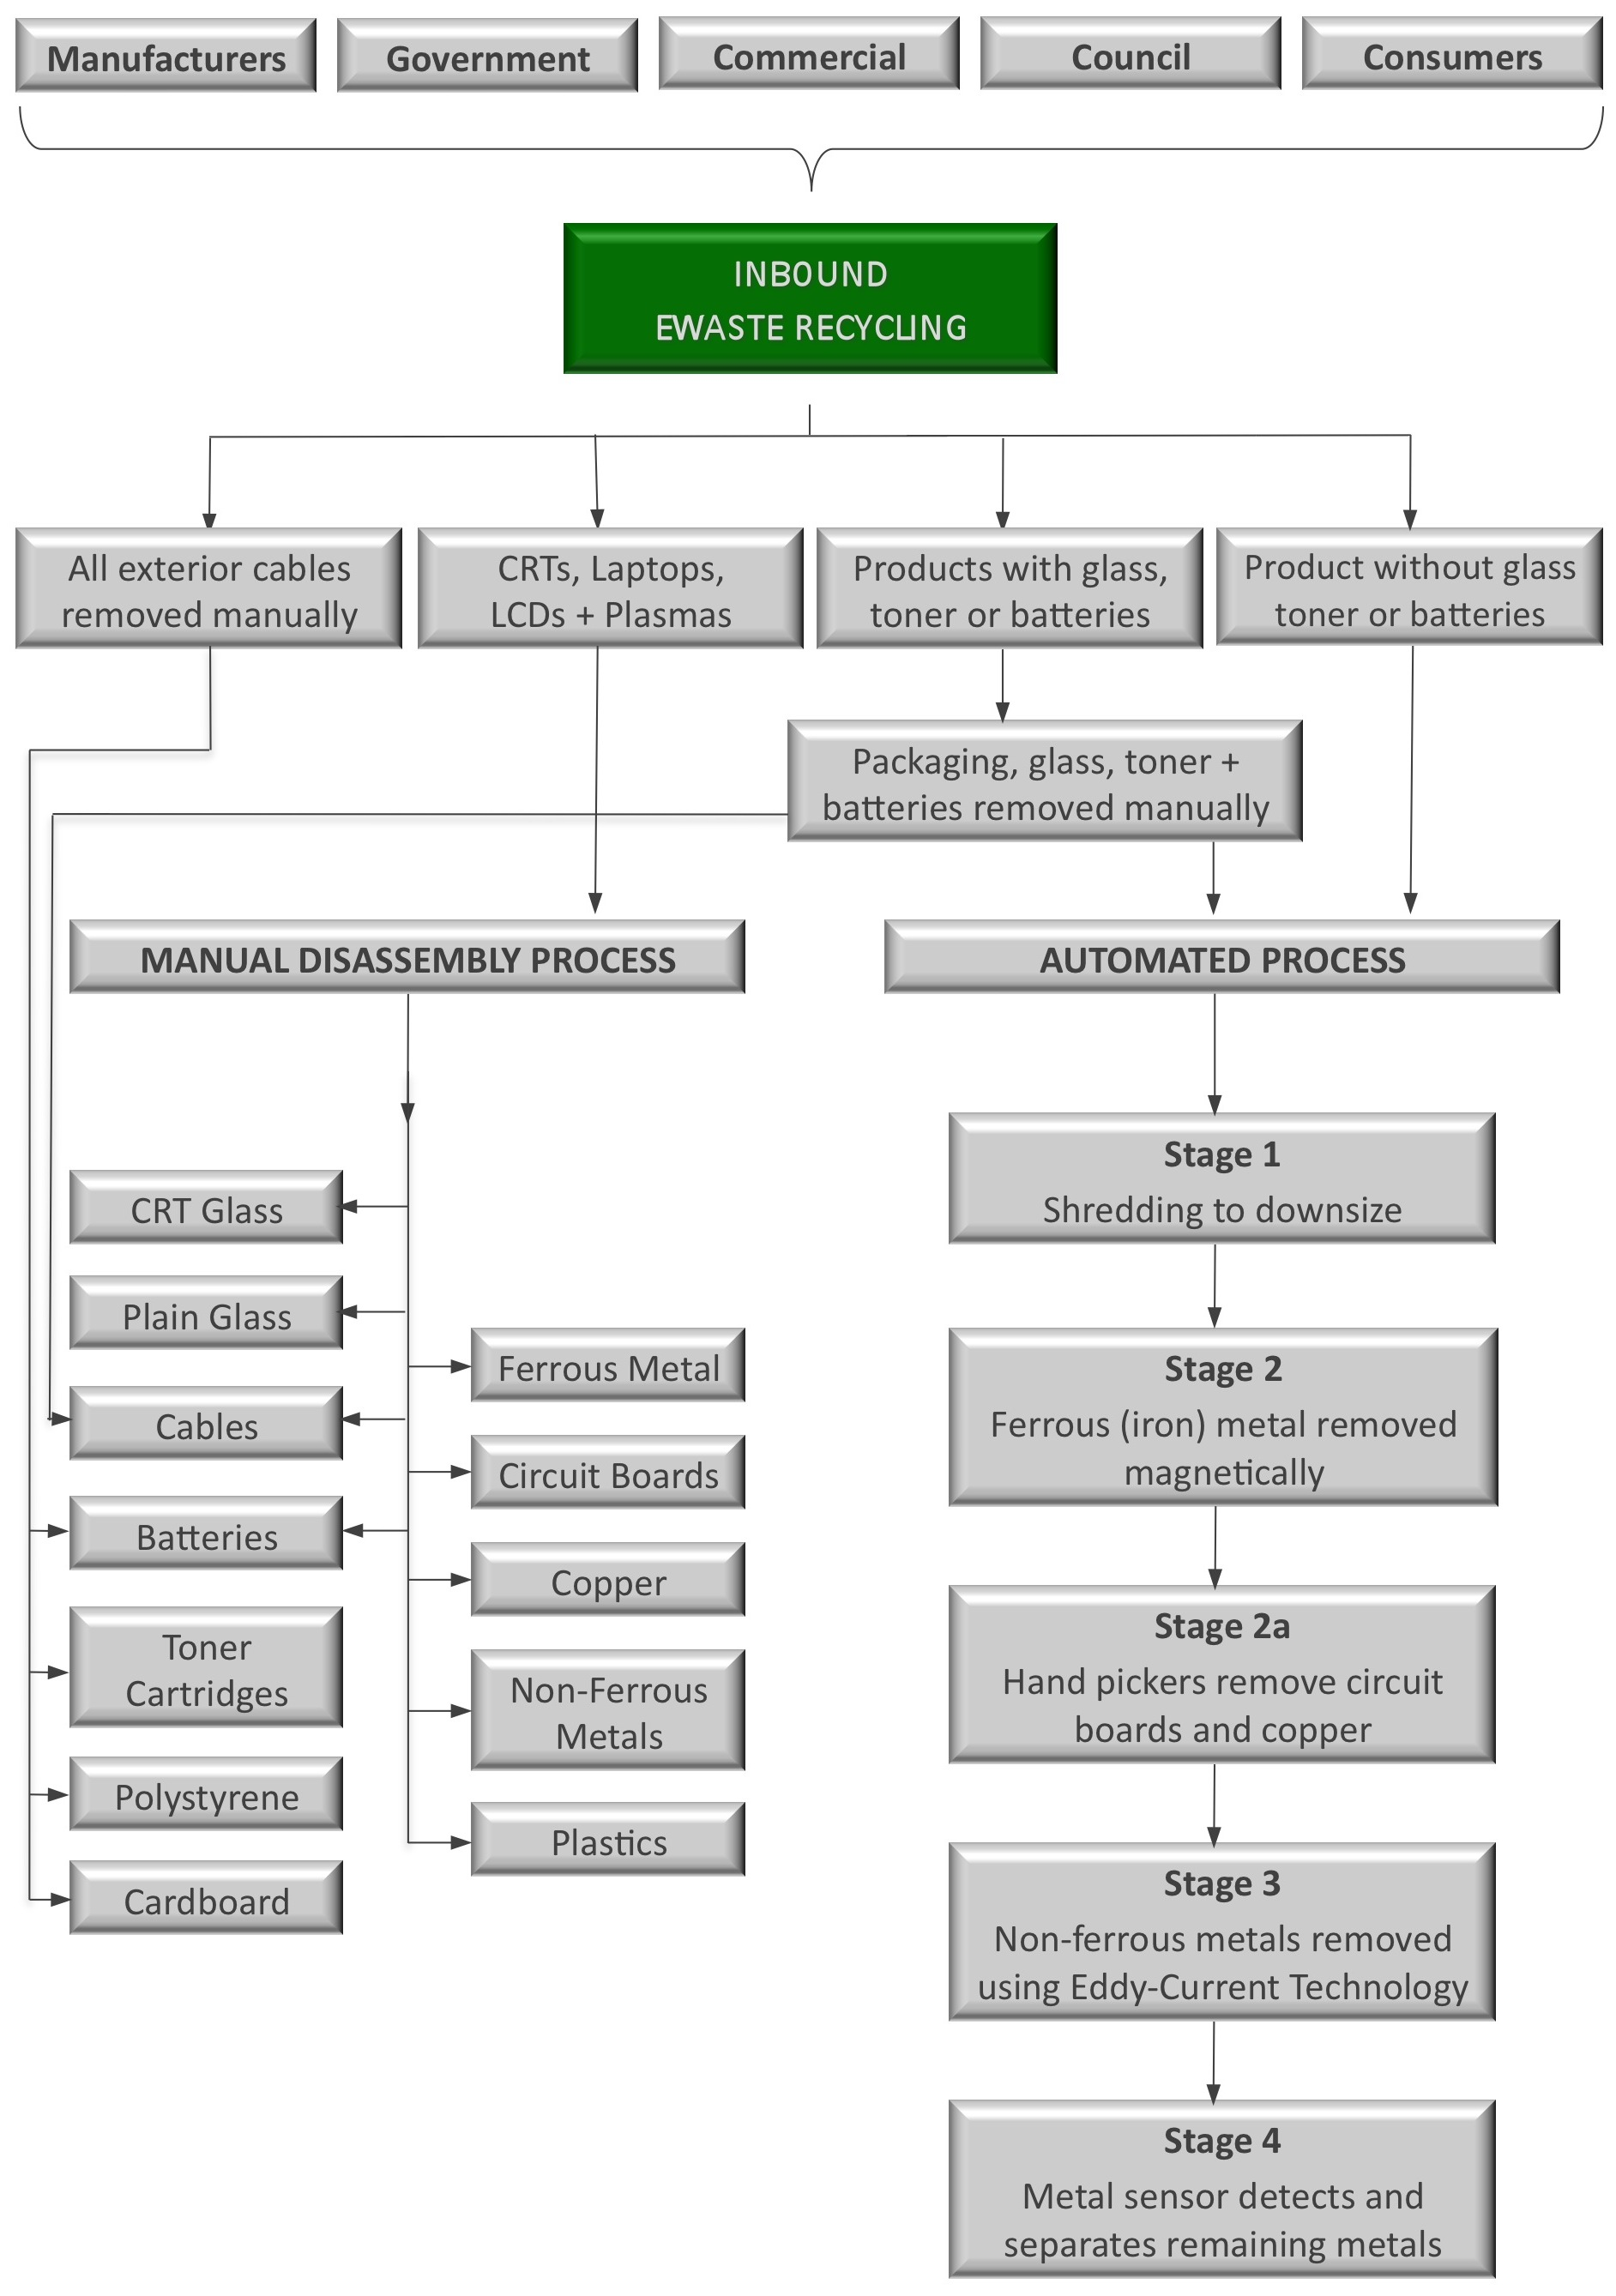
\includegraphics[width=0.8\textwidth]{img/recycling-process-flow-chart}
\caption{Diagrama de flujo del proceso de reciclado de la e-basura \cite{recycling-process}.}
\end{center}
\end{figure}

\begin{itemize}

\item{Todo comienza con la recolección de los dispositivos que contienen los elementos a reciclar y reutilizar. Este proceso debe involucrar a todos los agentes de la sociedad: empresas fabricantes, empresas y distribuidores que comercializan, gobiernos nacionales y locales y por supuesto al consumidor final. Deben establecerse los procedimientos sencillos para que el consumidor final pueda desechar de una forma cómoda todos aquellos dispositivos que no vaya a volver a utilizar y debe concienciarse al consumidor final de los beneficios de este acto comparándolo con el hecho de depositar en la basura normal estos dispositivos.}

\item{Una vez recogidos los dispositivos y trasladados a la planta de reciclaje, comienza un proceso de clasificación. Los dispositivos sin cristales, tóner o baterías son trasladados directamente a un proceso automático de desensamblado. El resto de dispositivos pasa previamente por una cadena de trabajo manual donde obreros especializados extraen todos los elementos reciclables y reusables y los clasifican: cables, cristal, baterías, circuitos integrados, materiales plásticos, aluminios y otros materiales, etc.}

\item{El proceso automático de desensamblado trata de separar los diferentes metales existentes en los componentes de forma automática basándose en las propiedades únicas de cada uno de los metales. Por ejemplo, el hierro es extraído a través de potentes electroimanes.}

\end{itemize}

Y ese es el resultado final de un proceso de reciclaje:

\begin{figure}[H]
\begin{center}
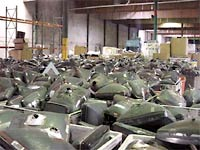
\includegraphics[]{img/ewaste_2}
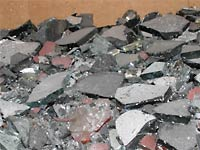
\includegraphics[]{img/ewaste_4}
\caption{Cristal de dispositivos CRT listo para ser reciclado y reutilizado.}
\end{center}
\end{figure}

\begin{figure}[H]
\begin{center}
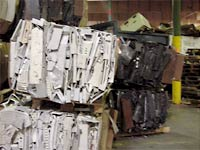
\includegraphics[]{img/ewaste_5}
\caption{Plástico compactado y empaquetado listo para ser reciclado y reutilizado.}
\end{center}
\end{figure}

\begin{figure}[H]
\begin{center}
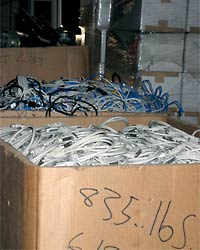
\includegraphics[]{img/ewaste_6}
\caption{Cables y otros componentes electrónicos listos para ser redistribuidos a otras compañías.}
\end{center}
\end{figure}

Tal y como se menciono anteriormente, este proceso no es sencillo y no es barato. Por ello, cada vez surgen más iniciativas y más procesos innovadores para tratar de abaratar los costes del mismo, realizarlo de forma más eficiente y favorecer cada vez más que estos procesos sean habituales en el nuestro día a día. Vamos a examinar dos de estas iniciativas:

\subsection{Invenovation, la completa industrialización del proceso de reutilización y reciclaje de e-basura.}

Innenovation \cite{invenovation} ha ideado un proceso que permite automatizar la recuperación de componentes de los dispositivos electrónicos tratando de minimizar al máximo la intervención humana con la consecuente reducción de costes e incremento de la eficiencia del proceso. 

Tal y como ellos mismos describen, su objetivo es recuperar de los dispositivos electrónicos todos los elementos base que luego pueden volver a ser utilizados para ensamblar nuevos dispositivos:

\begin{itemize}

\item{Resistencias.}
\item{Inductores.}
\item{Capacitores.}
\item{Circuitos integrados.}

\end{itemize}

Su idea se basa en que todos los dispositivos modernos se construyen a partir de estos bloques fundamentales y en su gran mayoría, todos estos bloques se unen a través de las placas de circuitos integrados mediante uniones a través de metales fundidos. El proceso de unión requiere calentar estos metales hasta que forman una conexión permanente entre la placa y el bloque al enfriarse. Para separarlos se puede seguir el mismo procedimiento y calentar esos metales hasta llevarlos a su estado líquido facilitando de esta manera la separación de los bloques anteriormente comentados. 

Su sistema, actualmente en prueba de concepto y buscando sponsor y patrocinadores, va a tratar una variedad de dispositivos muy amplia: móviles, ordenadores, etc. Por ello requiere de un sistema flexible para colocar las placas integradas en su sistema. En el gráfico siguiente se muestra el diseño con unos clips flexibles y ajustables que permiten sujetar la placa integrada en una rueda giratoria que se encargará de desplazar la placa por todo el sistema de desensamblado.

\begin{figure}[H]
\begin{center}
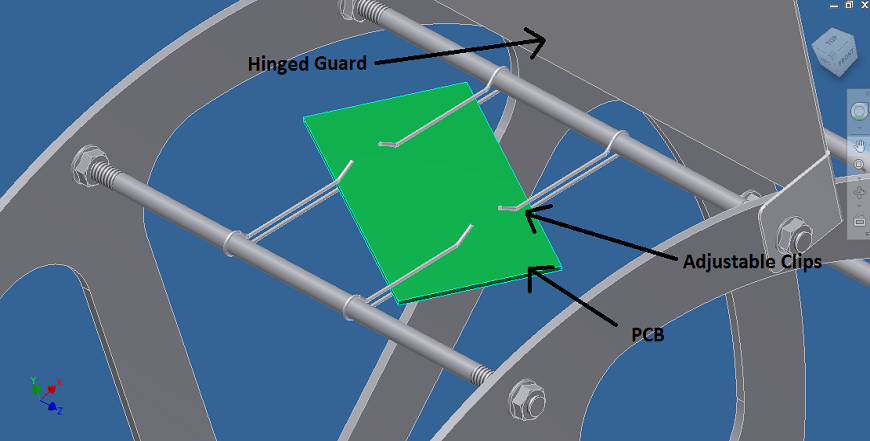
\includegraphics[width=0.8\textwidth]{img/D1}
\caption{Invenovation - sistema de sujeción de placas integradas \cite{invenovation}.}
\end{center}
\end{figure}

Una vez montadas las placas integradas en la rueda, son introducidas en un horno que calienta las placas a 200ºC/230ºC de forma controlada, tratando de reducir el stress térmico en los componentes, facilitando de este modo, su reutilización posterior. Los diferentes componentes van separándose poco a poco de la placa integrada.

\begin{figure}[H]
\begin{center}
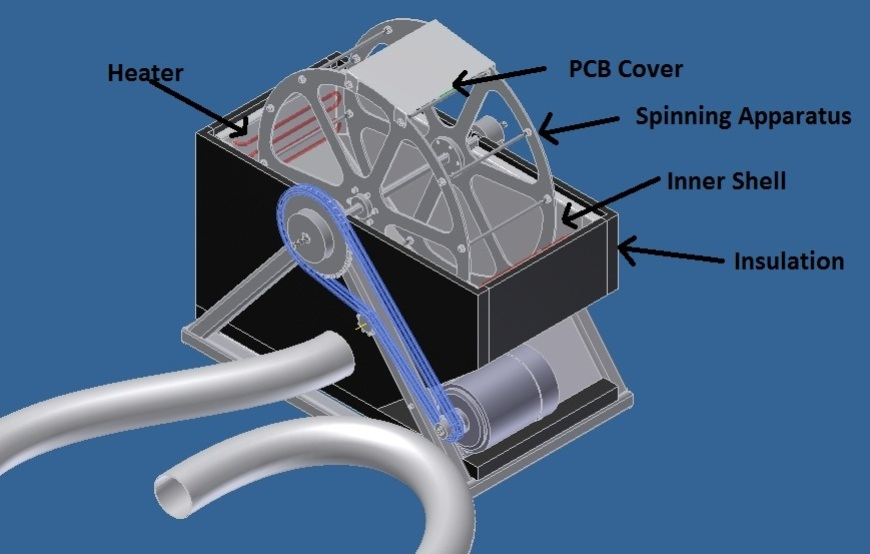
\includegraphics[width=0.8\textwidth]{img/D3}
\caption{Invenovation - horno de recuperación de componentes \cite{invenovation}.}
\end{center}
\end{figure}

\begin{figure}[H]
\begin{center}
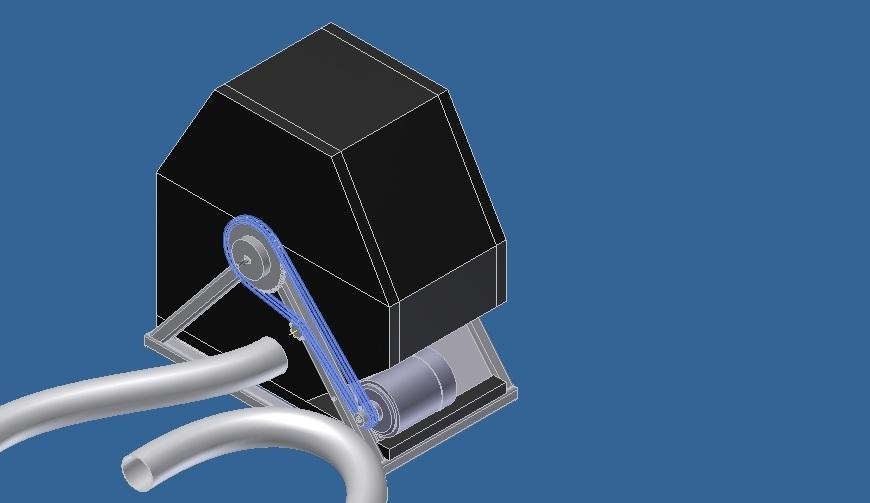
\includegraphics[width=0.8\textwidth]{img/D4}
\caption{Invenovation - horno de recuperación de componentes \cite{invenovation}.}
\end{center}
\end{figure}

\begin{figure}[H]
\begin{center}
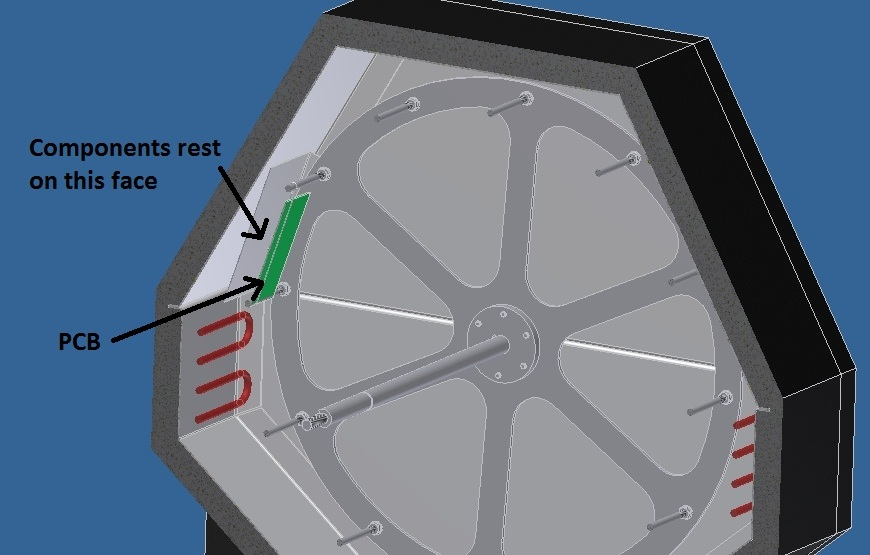
\includegraphics[width=0.8\textwidth]{img/D6}
\caption{Invenovation - horno de recuperación de componentes \cite{invenovation}.}
\end{center}
\end{figure}

Una vez que todos los componentes han sido separados de la placa, se introduce aire fresco en el horno para proceder a su enfriamiento y eliminar cualquier residuo tóxico que pudiera haberse desprendido. Una vez que se ha procedido a enfriar y eliminar los residuos tóxicos disminuye la velocidad de la rueda para permitir que los diferentes componentes salgan del sistema para ser trasladados a la siguiente etapa.

\begin{figure}[H]
\begin{center}
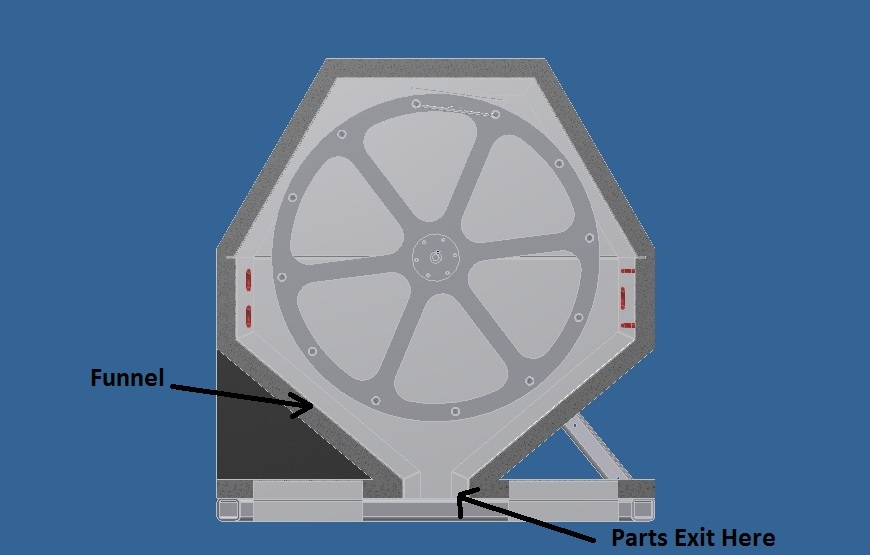
\includegraphics[width=0.8\textwidth]{img/D5}
\caption{Invenovation - horno de recuperación de componentes \cite{invenovation}.}
\end{center}
\end{figure}

Todos los componentes obtenidos pasan a la siguiente etapa del proceso, donde una combinación de sistemas de reconocimiento de formas asistido por ordenador se encargan de la clasificación de los diferentes componentes para separarlos, empaquetarlos y dejarlos listos para ser reutilizados.

\subsection{WEEE Advisory Board (WAB).}

En el año 2007, el Reino Unido creo el consejo WAB (Waste Electrical and Electronic Equipment) para ayudarles a definir las políticas y los diferentes procesos de reciclaje y reutilización de los dispositivos electrónicos que permitirían al Reino Unido situarse como uno de los países punteros en esta área.

El consejo estaba formado por 13 miembros de diferentes sectores: empresas de reciclaje, empresas fabricantes de dispositivos electrónicos, consultores medioambientales, etc. Su objetivo era ser una entidad independiente, solo el director general recibía un sueldo anual por parte del gobierno, para tratar de definir el sistema ideal de tratamiento de la e-basura.

Finalmente, la crisis económica que actualmente vivimos, ha podido con el objetivo inicialmente planteado, y el consejo ha sido disuelto, delegando sus funciones nuevamente en la actividad política estándar.

No obstante, durante su corto tiempo de vida, trabajaron en una especificación para la reutilización de la e-basura. En concreto, esta identificada como \emph{Public Available Specification (PAS) 141:2010. Specification for reuse of waste and used electrical and electronic equipment}. Esta especificación esta en estado borrador y su trabajo se ha discontinuado, pero es un ejemplo, de los intentos por estandarizar el tratamiento de la e-basura. El contenido de la misma pasa por obligar a las empresas que se encargan del teórico reciclaje a tomar determinadas medidas durante todo el proceso, de forma que los usuarios finales que adquieren dispositivos de segunda mano o ensamblados con componentes reutilizados, lo hagan con todas las garantías de seguridad. De entre todas las acciones de obligado cumplimiento destacan:

\begin{itemize}

\item{Inspección visual del componente.}
\item{Prueba de seguridad del circuito eléctrico.}
\item{Test de funcionamiento.}
\item{Eliminación de los datos.}
\item{Desensamblaje.}
\item{Reparación.}
\item{Limpieza.}

\end{itemize}

\begin{figure}[H]
\begin{center}
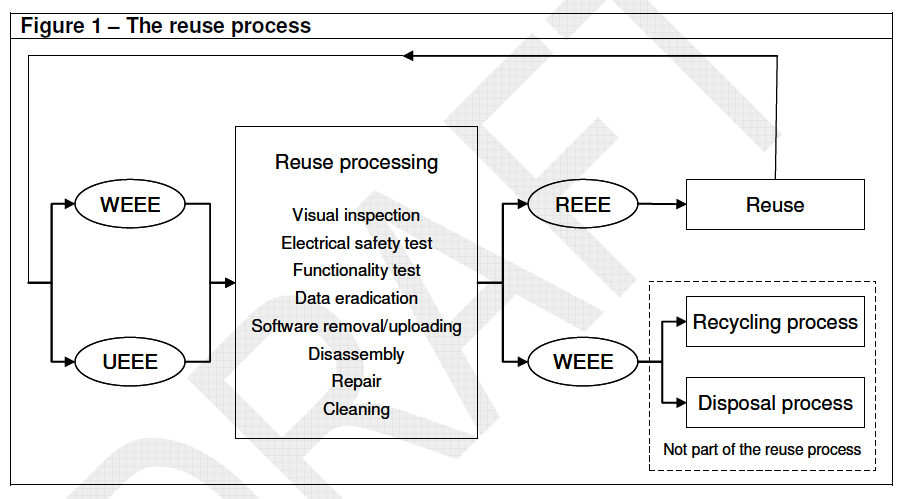
\includegraphics[width=0.8\textwidth]{img/reciclaje-weee}
\caption{Procedimiento a seguir según PAS 141:2010.}
\end{center}
\end{figure}

En la actualidad, las malas prácticas en estos procesos son habituales ya que permiten obtener beneficios económicos extra.